

There are two major ways  to perform the loading of a model, i.e., to provide  the platform with data :
\begin{itemize}
\item Loading a XML data file containing the complete or a part of the model
\item Creating a complete or a part of a model through the various API in C++ or C
\end{itemize}
It might also possible to adopt a mixed strategy to load a model. 


\begin{ndr}
  In all of these case, the question of the validity of a model is  posed. 
What is the validation procedure ?
\end{ndr}

These functionnalities are based of the implementation of two adjoint trees of object classes :
\begin{itemize}
\item The first tree, \texttt{SiconosModel}  is the core of the modelingTools and simulationsTools.
\item The second class tree \texttt{siconosModelXML} is devoted the XML Management and interfaces the external  library which implements the API DOM (libxml2).
\end{itemize}
This choice has been justified by the independance with  the external librairy of the XML management and the ability to extend easily the I/O for new derived object types.

\begin{ndr}
  Improve the justification of the choice of implementation 
\end{ndr}

In this chapter, we describe the implementation and the technical choices for the management of the input user's data and the creation of the model with these information. Particularly, the following are (must be) defined :
\begin{itemize}
\item Creation of the objects inside the class tree SiconosModel
\item Loading of the SiconosModel objects from the minimal data input
\item Linking of the object with the father and the child in the class tree SiconosModel 
\item Linking and loading of the SiconosModel objects from the SiconosModelXML
\item Creation of the objects inside the class tree SiconosModelXML
\item Loading of the SiconosModel objects from the XML data file
\item Linking of the object with the father and the child in the class tree SiconosModelXML
\item Description of some mixed loading Strategy (recall of the \ac{esd} normally !!) \S \ref{Sec:LoadingStrategy}
\item Save strategy of the SiconosModel tree
\item Save strategy of the SiconosModelXML tree
\item Validation strategy of the SiconosModel tree
\item Validation strategy of the SiconosModelXML tree
\end{itemize}


This first  part of chapter which explains  the model loading form the user poiut of view  must be reported in the \ac{sum}. 

\section{Model Loading Strategy}
\label{Sec:LoadingStrategy}


\subsection{Model loading from an  XML data file}

The reading of the file generate a DOM tree in memory with all the data. After that,  the creation of the SiconosModelXML tree is  based on this DOM tree.  The SiconosModelXML belongs to the SiconosModel object, which is the main object of the platform. From the SiconosModel,  the creation process is launched to build  all of the model. From this point, the Model creates the NSDS, which one creates the dynamical systems, ... The building is "top down" and gradually, with the Model at the top of the platform. 





\subsection{Creating and loading model through the API}

It is also  possible to create the objects of the platform without a XML file by using the API of the platform. The methods given to the users allow the creation of each object of the platform thanks to the constructors of each objects.


\subsection{Mixed strategies}


\section{Definition of three major types of construtors for the Siconosmodel objects.}

%% \subsection{The "create" methods}
%% The "create" functions have for goal to initialize the relating object. They fill its fields with XML data and link the objects belonging to it to their corresponding XML object, or, if the platform is manually built, only fill its fields with the data given in paramaters.


In this section, we define three majors types of constructors which must be defined and used in all classes of the platfrom for the creation of objects. In order to fix ideas, we consider a template objects of the form :

  {\ttfamily \raggedright \small
\#include\ <{}string>{}\\
\#include\ <{}vector>{}\\
\ \\
\ \\
using\ \textbf{namespace}\ std;\\
\ \\
\textbf{class}\ BaseObjectSiconos\ \{\\
\textbf{public}:\\
\ \ \ \ BaseObjectSiconos();\\
\ \ \ \ BaseObjectSiconos(\textbf{int}\ ii);\\
\ \ \ \ \textbf{void}\ display();\\
\ \ \ \ \textbf{void}\ fillObjectWithObjectXML();\\
\ \ \ \ \textbf{void}\ linkObjectXML();\\
\textbf{private}\ :\\
\ \ \textbf{int}\ i;\\
\ \ string\ type;\ \\
\};\\
\ \\
\ \\
\textbf{class}\ CompositionObject\\
\{\\
\ \textbf{public}:\\
\ \ \ \ CompositionObject();\\
\ \ \ \ CompositionObject(\textbf{int}\ ii);\\
\ \ \ \ \textbf{private}\ :\\
\ \ \textbf{int}\ i;\\
\};\\
\ \\
\textbf{class}\ ExternalObject\\
\{\\
\ \textbf{public}:\\
\ \ \ \ ExternalObject();\\
\ \ \ \ ExternalObject(\textbf{int}\ ii);\\
\ \ \ \ \textbf{private}\ :\\
\ \ \textbf{int}\ i;\\
\};\\
\ \\
\textbf{class}\ ObjectSiconosXML\ \\
\{\\
\textbf{public}\ :\\
\ \ \ \ ObjectSiconosXML();\\
\ \\
\textbf{private}\ :\\
\textsl{//\ Built-{}in\ types\ attributes\ (int,\ char,\ float,\ ..)}\\
\ \ \ string\ type;\ \\
\ \ \ \textbf{int}\ att;\\
\};\\
\ \\
\ \\
\textbf{class}\ ObjectSiconos\ :\ BaseObjectSiconos\\
\{\\
\textbf{public}\ :\\
ObjectSiconos();\\
ObjectSiconos(\textbf{int}\ aatt);\\
ObjectSiconos(ObjectSiconosXML\ $\ast$oxml);\\
\textbf{void}\ display();\\
\textbf{void}\ fillObjectWithObjectXML();\\
\textbf{void}\ linkObjectXML();\\
\ \\
\textbf{private}\ :\\
\textsl{//\ Built-{}in\ types\ attributes\ (int,\ char,\ float,\ ..)}\\
\ \ \ \ string\ type;\ \\
\ \ \ \textbf{int}\ att;\\
\ \\
\ \\
\textsl{//\ Objects\ members\ (Composition)}\\
\ \ \ CompositionObject\ compositionObject;\\
\ \\
\ \\
\textsl{//\ Pointer\ on\ external\ objects}\\
\ \ \ ObjectSiconosXML\ $\ast$objectsiconosxml;\\
\ \ \ ExternalObject\ $\ast$externalObject;\\
\ \\
\};\\
\ \\
\ \\
 }
\normalfont\normalsize


%% \begin{lstlisting}[frame=single,caption={Template objects}]
%% Class ObjectSiconos: BaseObjectSiconos
%% {
%% public :
%% ObjectSiconos();
%% ...

%% private :
%% // Built-in types attributes (int, char, float, ..)
%%    string type;
%%    AttType att;
%%    ...

%% // Objects members (Composition)
%%    CompositionObject compositionObject;
%%    ...

%% // Pointer on external objects
%%    ObjectSiconosXML *objectsiconosxml;
%%    ExternalObject *externalObject;
%%    ...
   
%% }
%% \end{lstlisting} 





\subsection{The Default Constructor}

The default constructor performs the following operations :
{\ttfamily \raggedright \small
\#include\ "{}SiconosObject.h"{}\\
\#include\ <{}iostream>{}\\
\ \\
\ \\
ObjectSiconos::ObjectSiconos():\\
\ \ \textsl{//\ Construtors\ of\ the\ Base\ Class}\\
\ \ \ \ BaseObjectSiconos(),\\
\ \ \textsl{//\ Constructors\ of\ the\ Built-{}in\ types}\\
\ \ \ \ type("{}OBJECTSICONOS\underline\ TYPE"{}),att(0),\\
\ \ \textsl{//\ Constructors\ of\ the\ object\ members\ (composition)}\\
\ \ \ \ compositionObject()\\
\{\\
\ \ cout\ <{}<{}\ "{}ObjectSiconos\ -{}-{}\ \textbf{default}\ Constructor"{}\ <{}<{}\ endl;\\
\ \ \\
\ \ \textsl{//\ Initialization\ of\ pointers\ on\ external\ objects}\\
\ \ objectsiconosxml\ =0;\\
\ \ externalObject\ =0;\\
\ \ \\
\ \ \textsl{//\ Do\ we\ need\ to\ call\ the\ new\ operator\ ?}\\
\ \ \textsl{//\ externalObject\ =\ new\ ExternalObject();}\\
\}\\
\ \\
BaseObjectSiconos::BaseObjectSiconos():i(0),type("{}BASE\underline\ TYPE"{})\\
\ \ \ \ \{\ \\
\ \ \ \ \ \ cout\ <{}<{}\ "{}BaseObjectSiconos\ -{}-{}\ \textbf{default}\ Constructor"{}\ <{}<{}\ endl;\\
\ \ \ \ \}\\
\ \\
CompositionObject::CompositionObject():i(0)\\
\ \ \ \ \{\\
\ \ \ \ \};\\
\ \\
ExternalObject::ExternalObject():i(0)\\
\ \ \ \ \{\\
\ \ \ \ \}\\
\ \\
\ \\
 }
\normalfont\normalsize






%% \begin{lstlisting}[frame=single,caption={Default Constructor}]
%% ObjectSiconos::ObjectSiconos() :
%%    // Call explicitely one constructors of the base Object
%%    BaseObjectSiconos(...);
%%    // Call explicitely one constructors of the members
%%    // Built-in types attributes
%%    type("OBJECT_TYPE"), att(defaultvalue),
%%    //Object members :
%%    compositionObject(newDefaultValueIfNeccesary), ...
%%    {
%%    Initialization of pointers on external objects
%%    this->objectsiconosXML = 0 ;  // ObjectXML pointer
%%    this->externalObject = 0;

%%    // Do we need to call the new operator ?
%%     externalObject = new ExternalObject();
%%    }
%% \end{lstlisting} 

\begin{ndr}
  \begin{enumerate}
  \item Remove init() method !!!! This is the role of the Default constructor.
  \item Do we need to use the new operator if the sizes of the object are not defined ? What is the interest to call the Default constructor with a new ?
  \end{enumerate}

\end{ndr}

\subsection{Constructor from the mininal data}

This constructor performs  the contruction of a object through given a minimal set of data.  It is composed of the following operations :
{\ttfamily \raggedright \small
\#include\ "{}SiconosObject.h"{}\\
\#include\ <{}iostream>{}\\
\ \\
ObjectSiconos::ObjectSiconos(\textbf{int}\ aatt,\ string\ ttype):\\
\ \ \textsl{//\ Construtors\ of\ the\ Base\ Class}\\
BaseObjectSiconos(2$\ast$aatt),\\
\ \ \textsl{//\ Constructors\ of\ the\ Built-{}in\ types}\\
type(ttype),att(aatt),\\
\ \ \textsl{//\ Constructors\ of\ the\ object\ members\ (composition)}\\
compositionObject(5$\ast$aatt)\\
\{\\
\ \ cout\ <{}<{}\ "{}ObjectSiconos\ -{}-{}\ Constructor\ with\ minimal\ data"{}\ <{}<{}\ endl;\\
\ \ \textsl{//\ ObjectSiconos();\ //\ Dangerous\ Fix\ the\ order\ ??}\\
\ \ \textsl{//\ Initialization\ of\ pointers\ on\ external\ objects}\\
\ \ objectsiconosxml\ =0;\\
\ \ externalObject\ =\ \textbf{new}\ ExternalObject(aatt);\\
\}\\
\ \\
CompositionObject::CompositionObject(\textbf{int}\ ii):i(ii)\\
\ \ \ \ \{\\
\ \ \ \ \};\\
\ \\
\ \\
ExternalObject::ExternalObject(\textbf{int}\ ii):i(ii)\\
\ \ \ \ \{\\
\ \ \ \ \}\\
\ \\
BaseObjectSiconos::BaseObjectSiconos(\textbf{int}\ ii):i(ii),type("{}BASE\underline\ TYPE"{})\\
\ \ \ \ \{\ \\
\ \ \ \ \ \ cout\ <{}<{}\ "{}BaseObjectSiconos\ -{}-{}\ \textbf{default}\ Constructor"{}\ <{}<{}\ endl;\\
\ \ \ \ \}\\
\ \\
 }
\normalfont\normalsize


%% \begin{lstlisting}[frame=single,caption={Constructor from the mininal data}]
%% Object::object(AttributeType1 data1,...,AttributeTypeN dataN )
%%    {
%%    Object(); // Default constructor

%%    // Loading of Simple type attributes
%%    this->attribute1 = data1 ; //loading of the attributes
%%    ....
%%    this->attributeN = dataN ;

%%    //Object attributes

%%    // if data are present for this object call the specific constructor
%%    attributeObject1 = new AttributeObject1type(data11, data 1N);

%%    // if not, do we need to call the default constructor (new needed ?)
%%    attributeObject1 = new AttributeObject1type();
%%    // XML Management, node creation, and link downwards ? see NDR below
%%    }
%% \end{lstlisting} 

 \begin{ndr}
   \begin{enumerate}
   \item Be careful of the conflict between the new in the Default Constructor and in this constructor, if a new is called in the default Constructor
   \item Define if the object in attributes must created now of after and then link
   \item Define the procedure for the XML management :
     \begin{itemize}
     \item  Where  is the constructor of the assciated ObjectXML ? 
     \item  Use of the SaveObjectXML ?
     \item  Creation of XML sub -tree ? Advantages : Don't need to know what is the father node to fullfill a node at the moment of construction
     \end{itemize}
   \end{enumerate}
 \end{ndr}


\subsection{Constructor from the ObjectXML of the SiconosModelXML tree}

This constructor performs  the contruction of a object given a XML node. there is two steps in this type of contruction  based on the two-associted objetcs, i.e, Object, ObjectXML (for instance, DynamicalSystem and DynamicalSystemXML). The first one is the loading of the ObjectXML from the XML node.Tis step will be detailed in the section \ref{Sec:XMLnode}. The second  step is the loading of the attributes of the object from the ObjectXML. The operations are described in the Listing~\ref{ConstructorObjectXML}.

{\ttfamily \raggedright \small
\#include\ "{}SiconosObject.h"{}\\
\#include\ <{}iostream>{}\\
\ \\
ObjectSiconos::ObjectSiconos(ObjectSiconosXML\ $\ast$objectsiconosxml):\\
\ \ \textsl{//\ Construtors\ of\ the\ Base\ Class}\\
BaseObjectSiconos(),\\
\ \ \textsl{//\ Constructors\ of\ the\ Built-{}in\ types}\\
type("{}OBJETSICONOS\underline\ TYPE"{}),att(),\\
\ \ \textsl{//\ Constructors\ of\ the\ object\ members\ (composition)}\\
compositionObject()\\
\{\\
\ \ cout\ <{}<{}\ "{}ObjectSiconos\ -{}-{}\ Constructor\ with\ minimal\ data"{}\ <{}<{}\ endl;\\
\ \ \textsl{//\ ObjectSiconos();\ //\ Dangerous\ Fix\ the\ order\ ??}\\
\ \ \textsl{//\ Initialization\ of\ pointers\ on\ external\ objects}\\
\ \\
\ \ objectsiconosxml\ =\ oxml;\\
\ \ \textsl{//\ Loading\ of\ the\ attribute\ from\ the\ ObjectXML}\\
\ \ fillObjectWithObjectXML();\\
\ \ \textsl{//\ Create\ from\ factory\ if\ needed\ (new)\ and\ \ link\ downwards\ the\ External\ objects}\\
\ \ linkObjectXML();\\
\ \\
\}\\
\ \\
 }
\normalfont\normalsize


%% \begin{lstlisting}[frame=single,caption={Constructor from the ObjectXML of the SiconosModelXML tree }, label={ConstructorObjectXML}]
%% Object::Object(ObjectXML objectxml)
%%    {
%%     Object(); // Default constructor
%%     this->objectxml = objectXML;        
%%     this->fillObjectWithDSXML(); // Loading of the attribute from the ObjectXML
%%     this->linkObjectXML();       // Link downwards
%%    }
%% \end{lstlisting} 



 \begin{ndr}
   \begin{enumerate}
   \item Define the procedure for the XML management of the child :
     \begin{itemize}
     \item The constructor for the Child Object (Externalobject) is in the link ?
     \end{itemize}
   \item Perhaps rename the method fill and link, or include it directly in the constructor ?
   \end{enumerate}
 \end{ndr}

\clearpage

%{\ttfamily \raggedright \small
ObjectSiconos::ObjectSiconos():BaseObjectSiconos(),type("{}DERIVED\underline\ TYPE"{}),att(100),\ compositionObject()\\
\{\\
\ \ cout\ <{}<{}\ "{}ObjectSiconos\ -{}-{}\ default\ Constructor"{}\ <{}<{}\ endl;\\
\ \ objectsiconosxml\ =0;\\
\ \ externalObject\ =0;\\
\}\\
\ \\
\ \\
ObjectSiconos::ObjectSiconos(int\ aatt,\ string\ ttype):BaseObjectSiconos(),type(ttype),att(aatt),\ compositionObject()\\
\{\\
\ \ cout\ <{}<{}\ "{}ObjectSiconos\ -{}-{}\ Constructor\ with\ minimal\ data"{}\ <{}<{}\ endl;\\
\ \ ObjectSiconos();\ \textsl{//\ Fix\ the\ order\ ??}\\
\ \ externalObject\ =\ new\ ExternalObject(aatt);\\
\}\\
\ void\ ObjectSiconos::display()\\
\{\\
\ \ \textsl{//Do\ we\ need\ to\ call\ it\ inside\ the\ braces\ ?}\\
\ \ BaseObjectSiconos::display();\ \\
\ \ cout\ <{}<{}\ this-{}>{}att\ <{}<{}\ endl;\\
\ \ cout\ <{}<{}\ this-{}>{}type\ <{}<{}\ endl;\\
\}\\
\ \\
\ \\
ObjectSiconosXML::ObjectSiconosXML():type("{}TYPE"{}),att(100)\\
\{\\
\}\\
\ \\
\ \\
CompositionObject::CompositionObject():i(0)\\
\ \ \ \ \{\\
\ \ \ \ \};\\
CompositionObject::CompositionObject(int\ ii)\\
\ \ \ \ \{\\
\ \ \ \ \ \ i\ =ii;\\
\ \ \ \ \};\\
\ \\
ExternalObject::ExternalObject():i(0)\\
\ \ \ \ \{\\
\ \ \ \ \}\\
ExternalObject::ExternalObject(int\ ii)\\
\ \ \ \ \{\\
\ \ \ \ \ \ i=\ ii;\\
\ \ \ \ \}\\
\ \\
\ \\
int\ main(void)\\
\ \\
\{\\
\ \\
\ \ ObjectSiconos\ o1;\\
\ \ o1.display();\\
\ \ \\
\ \\
\ \\
\ \ ObjectSiconos\ o2(10,"{}derived\underline\ TYPE"{});\\
\ \ o2.display();\\
\}\\
\ \\
 }
\normalfont\normalsize

{\ttfamily \raggedright \small
\#include\ "{}SiconosObject.h"{}\\
\#include\ <{}iostream>{}\\
\ \\
\ \\
BaseObjectSiconos::BaseObjectSiconos():i(0),type("{}BASE\underline\ TYPE"{})\\
\ \ \ \ \{\ \\
\ \ \ \ \ \ cout\ <{}<{}\ "{}BaseObjectSiconos\ -{}-{}\ default\ Constructor"{}\ <{}<{}\ endl;\\
\ \ \ \ \}\\
void\ BaseObjectSiconos::display()\\
\ \ \ \ \{\\
\ \ \ \ \ \ cout\ <{}<{}\ this-{}>{}i\ <{}<{}\ endl;\\
\ \ \ \ \ \ cout\ <{}<{}\ this-{}>{}type\ <{}<{}\ endl;\\
\ \ \ \ \}\\
\ \\
\ \\
\ \\
ObjectSiconos::ObjectSiconos():BaseObjectSiconos(),type("{}DERIVED\underline\ TYPE"{}),att(100),\ compositionObject()\\
\{\\
\ \ cout\ <{}<{}\ "{}ObjectSiconos\ -{}-{}\ default\ Constructor"{}\ <{}<{}\ endl;\\
\ \ objectsiconosxml\ =0;\\
\ \ externalObject\ =0;\\
\}\\
\ \\
\ \\
ObjectSiconos::ObjectSiconos(int\ aatt,\ string\ ttype):BaseObjectSiconos(),type(ttype),att(aatt),\ compositionObject()\\
\{\\
\ \ cout\ <{}<{}\ "{}ObjectSiconos\ -{}-{}\ Constructor\ with\ minimal\ data"{}\ <{}<{}\ endl;\\
\ \ ObjectSiconos();\ \textsl{//\ Fix\ the\ order\ ??}\\
\ \ externalObject\ =\ new\ ExternalObject(aatt);\\
\}\\
\ void\ ObjectSiconos::display()\\
\{\\
\ \ \textsl{//Do\ we\ need\ to\ call\ it\ inside\ the\ braces\ ?}\\
\ \ BaseObjectSiconos::display();\ \\
\ \ cout\ <{}<{}\ this-{}>{}att\ <{}<{}\ endl;\\
\ \ cout\ <{}<{}\ this-{}>{}type\ <{}<{}\ endl;\\
\}\\
\ \\
\ \\
ObjectSiconosXML::ObjectSiconosXML():type("{}TYPE"{}),att(100)\\
\{\\
\}\\
\ \\
\ \\
CompositionObject::CompositionObject():i(0)\\
\ \ \ \ \{\\
\ \ \ \ \};\\
CompositionObject::CompositionObject(int\ ii)\\
\ \ \ \ \{\\
\ \ \ \ \ \ i\ =ii;\\
\ \ \ \ \};\\
\ \\
ExternalObject::ExternalObject():i(0)\\
\ \ \ \ \{\\
\ \ \ \ \}\\
ExternalObject::ExternalObject(int\ ii)\\
\ \ \ \ \{\\
\ \ \ \ \ \ i=\ ii;\\
\ \ \ \ \}\\
\ \\
\ \\
int\ main(void)\\
\ \\
\{\\
\ \\
\ \ ObjectSiconos\ o1;\\
\ \ o1.display();\\
\ \ \\
\ \\
\ \\
\ \ ObjectSiconos\ o2(10,"{}derived\underline\ TYPE"{});\\
\ \ o2.display();\\
\}\\
\ \\
 }
\normalfont\normalsize

{\ttfamily \raggedright \small
\ \\
\ \\
\ \\
\ \\
\ \\
\ \\
\ \\
\ \\
\ \\
\ \\
\ \\
\ \\
\ \\
\ \\
\ \\
\ \\
\ \\
\#include\ "{}SiconosObject.h"{}\\
\#include\ <{}iostream>{}\\
\ \\
\ \\
BaseObjectSiconos::BaseObjectSiconos():i(0),type("{}BASE\underline\ TYPE"{})\\
\ \ \ \ \{\ \\
\ \ \ \ \ \ cout\ <{}<{}\ "{}BaseObjectSiconos\ -{}-{}\ \textbf{default}\ Constructor"{}\ <{}<{}\ endl;\\
\ \ \ \ \}\\
\textbf{void}\ BaseObjectSiconos::display()\\
\ \ \ \ \{\\
\ \ \ \ \ \ cout\ <{}<{}\ \textbf{this}-{}>{}i\ <{}<{}\ endl;\\
\ \ \ \ \ \ cout\ <{}<{}\ \textbf{this}-{}>{}type\ <{}<{}\ endl;\\
\ \ \ \ \}\\
\ \\
\ \\
\ \\
ObjectSiconos::ObjectSiconos():BaseObjectSiconos(),type("{}DERIVED\underline\ TYPE"{}),att(100),\ compositionObject()\\
\{\\
\ \ cout\ <{}<{}\ "{}ObjectSiconos\ -{}-{}\ \textbf{default}\ Constructor"{}\ <{}<{}\ endl;\\
\ \ objectsiconosxml\ =0;\\
\ \ externalObject\ =0;\\
\}\\
\ \\
\ \\
ObjectSiconos::ObjectSiconos(\textbf{int}\ aatt,\ string\ ttype):BaseObjectSiconos(),type(ttype),att(aatt),\ compositionObject()\\
\{\\
\ \ cout\ <{}<{}\ "{}ObjectSiconos\ -{}-{}\ Constructor\ with\ minimal\ data"{}\ <{}<{}\ endl;\\
\ \ ObjectSiconos();\ \textsl{//\ Fix\ the\ order\ ??}\\
\ \ externalObject\ =\ \textbf{new}\ ExternalObject(aatt);\\
\}\\
\ \textbf{void}\ ObjectSiconos::display()\\
\{\\
\ \ \textsl{//Do\ we\ need\ to\ call\ it\ inside\ the\ braces\ ?}\\
\ \ BaseObjectSiconos::display();\ \\
\ \ cout\ <{}<{}\ \textbf{this}-{}>{}att\ <{}<{}\ endl;\\
\ \ cout\ <{}<{}\ \textbf{this}-{}>{}type\ <{}<{}\ endl;\\
\}\\
\ \\
\ \\
ObjectSiconosXML::ObjectSiconosXML():type("{}TYPE"{}),att(100)\\
\{\\
\}\\
\ \\
\ \\
CompositionObject::CompositionObject():i(0)\\
\ \ \ \ \{\\
\ \ \ \ \};\\
CompositionObject::CompositionObject(\textbf{int}\ ii)\\
\ \ \ \ \{\\
\ \ \ \ \ \ i\ =ii;\\
\ \ \ \ \};\\
\ \\
ExternalObject::ExternalObject():i(0)\\
\ \ \ \ \{\\
\ \ \ \ \}\\
ExternalObject::ExternalObject(\textbf{int}\ ii)\\
\ \ \ \ \{\\
\ \ \ \ \ \ i=\ ii;\\
\ \ \ \ \}\\
\ \\
\ \\
\textbf{int}\ main(\textbf{void})\\
\ \\
\{\\
\ \\
\ \ ObjectSiconos\ o1;\\
\ \ o1.display();\\
\ \ \\
\ \\
\ \\
\ \ ObjectSiconos\ o2(10,"{}derived\underline\ TYPE"{});\\
\ \ o2.display();\\
\}\\
\ \\
 }
\normalfont\normalsize

{\ttfamily \raggedright \small
\ \\
\ \\
\ \\
\ \\
\ \\
\ \\
\ \\
\ \\
\ \\
\ \\
\ \\
\ \\
\ \\
\ \\
\ \\
\ \\
\ \\
\#include\ "{}SiconosObject.h"{}\\
\#include\ <{}iostream>{}\\
\ \\
\ \\
BaseObjectSiconos::BaseObjectSiconos():i(0),type("{}BASE\underline\ TYPE"{})\\
\ \ \ \ \{\ \\
\ \ \ \ \ \ cout\ <{}<{}\ "{}BaseObjectSiconos\ -{}-{}\ \textbf{default}\ Constructor"{}\ <{}<{}\ endl;\\
\ \ \ \ \}\\
\textbf{void}\ BaseObjectSiconos::display()\\
\ \ \ \ \{\\
\ \ \ \ \ \ cout\ <{}<{}\ \textbf{this}-{}>{}i\ <{}<{}\ endl;\\
\ \ \ \ \ \ cout\ <{}<{}\ \textbf{this}-{}>{}type\ <{}<{}\ endl;\\
\ \ \ \ \}\\
\ \\
\ \\
\ \\
ObjectSiconos::ObjectSiconos():BaseObjectSiconos(),type("{}DERIVED\underline\ TYPE"{}),att(100),\ compositionObject()\\
\{\\
\ \ cout\ <{}<{}\ "{}ObjectSiconos\ -{}-{}\ \textbf{default}\ Constructor"{}\ <{}<{}\ endl;\\
\ \ objectsiconosxml\ =0;\\
\ \ externalObject\ =0;\\
\}\\
\ \\
\ \\
ObjectSiconos::ObjectSiconos(\textbf{int}\ aatt,\ string\ ttype):BaseObjectSiconos(),type(ttype),att(aatt),\ compositionObject()\\
\{\\
\ \ cout\ <{}<{}\ "{}ObjectSiconos\ -{}-{}\ Constructor\ with\ minimal\ data"{}\ <{}<{}\ endl;\\
\ \ ObjectSiconos();\ \textsl{//\ Fix\ the\ order\ ??}\\
\ \ externalObject\ =\ \textbf{new}\ ExternalObject(aatt);\\
\}\\
\ \textbf{void}\ ObjectSiconos::display()\\
\{\\
\ \ \textsl{//Do\ we\ need\ to\ call\ it\ inside\ the\ braces\ ?}\\
\ \ BaseObjectSiconos::display();\ \\
\ \ cout\ <{}<{}\ \textbf{this}-{}>{}att\ <{}<{}\ endl;\\
\ \ cout\ <{}<{}\ \textbf{this}-{}>{}type\ <{}<{}\ endl;\\
\}\\
\ \\
\ \\
ObjectSiconosXML::ObjectSiconosXML():type("{}TYPE"{}),att(100)\\
\{\\
\}\\
\ \\
\ \\
CompositionObject::CompositionObject():i(0)\\
\ \ \ \ \{\\
\ \ \ \ \};\\
CompositionObject::CompositionObject(\textbf{int}\ ii)\\
\ \ \ \ \{\\
\ \ \ \ \ \ i\ =ii;\\
\ \ \ \ \};\\
\ \\
ExternalObject::ExternalObject():i(0)\\
\ \ \ \ \{\\
\ \ \ \ \}\\
ExternalObject::ExternalObject(\textbf{int}\ ii)\\
\ \ \ \ \{\\
\ \ \ \ \ \ i=\ ii;\\
\ \ \ \ \}\\
\ \\
\ \\
\textbf{int}\ main(\textbf{void})\\
\ \\
\{\\
\ \\
\ \ ObjectSiconos\ o1;\\
\ \ o1.display();\\
\ \ \\
\ \\
\ \\
\ \ ObjectSiconos\ o2(10,"{}derived\underline\ TYPE"{});\\
\ \ o2.display();\\
\}\\
\ \\
 }
\normalfont\normalsize

{\ttfamily \raggedright \small
\ \\
\ \\
\ \\
\ \\
\ \\
\ \\
\ \\
\ \\
\ \\
\ \\
\ \\
\ \\
\ \\
\ \\
\ \\
\ \\
\ \\
\#include\ "{}SiconosObject.h"{}\\
\#include\ <{}iostream>{}\\
\ \\
\ \\
BaseObjectSiconos::BaseObjectSiconos():i(0),type("{}BASE\underline\ TYPE"{})\\
\ \ \ \ \{\ \\
\ \ \ \ \ \ cout\ <{}<{}\ "{}BaseObjectSiconos\ -{}-{}\ \textbf{default}\ Constructor"{}\ <{}<{}\ endl;\\
\ \ \ \ \}\\
\textbf{void}\ BaseObjectSiconos::display()\\
\ \ \ \ \{\\
\ \ \ \ \ \ cout\ <{}<{}\ \textbf{this}-{}>{}i\ <{}<{}\ endl;\\
\ \ \ \ \ \ cout\ <{}<{}\ \textbf{this}-{}>{}type\ <{}<{}\ endl;\\
\ \ \ \ \}\\
\ \\
\ \\
\ \\
ObjectSiconos::ObjectSiconos():BaseObjectSiconos(),type("{}DERIVED\underline\ TYPE"{}),att(100),\ compositionObject()\\
\{\\
\ \ cout\ <{}<{}\ "{}ObjectSiconos\ -{}-{}\ \textbf{default}\ Constructor"{}\ <{}<{}\ endl;\\
\ \ objectsiconosxml\ =0;\\
\ \ externalObject\ =0;\\
\}\\
\ \\
\ \\
ObjectSiconos::ObjectSiconos(\textbf{int}\ aatt,\ string\ ttype):BaseObjectSiconos(),type(ttype),att(aatt),\ compositionObject()\\
\{\\
\ \ cout\ <{}<{}\ "{}ObjectSiconos\ -{}-{}\ Constructor\ with\ minimal\ data"{}\ <{}<{}\ endl;\\
\ \ ObjectSiconos();\ \textsl{//\ Fix\ the\ order\ ??}\\
\ \ externalObject\ =\ \textbf{new}\ ExternalObject(aatt);\\
\}\\
\ \textbf{void}\ ObjectSiconos::display()\\
\{\\
\ \ \textsl{//Do\ we\ need\ to\ call\ it\ inside\ the\ braces\ ?}\\
\ \ BaseObjectSiconos::display();\ \\
\ \ cout\ <{}<{}\ \textbf{this}-{}>{}att\ <{}<{}\ endl;\\
\ \ cout\ <{}<{}\ \textbf{this}-{}>{}type\ <{}<{}\ endl;\\
\}\\
\ \\
\ \\
ObjectSiconosXML::ObjectSiconosXML():type("{}TYPE"{}),att(100)\\
\{\\
\}\\
\ \\
\ \\
CompositionObject::CompositionObject():i(0)\\
\ \ \ \ \{\\
\ \ \ \ \};\\
CompositionObject::CompositionObject(\textbf{int}\ ii)\\
\ \ \ \ \{\\
\ \ \ \ \ \ i\ =ii;\\
\ \ \ \ \};\\
\ \\
ExternalObject::ExternalObject():i(0)\\
\ \ \ \ \{\\
\ \ \ \ \}\\
ExternalObject::ExternalObject(\textbf{int}\ ii)\\
\ \ \ \ \{\\
\ \ \ \ \ \ i=\ ii;\\
\ \ \ \ \}\\
\ \\
\ \\
\textbf{int}\ main(\textbf{void})\\
\ \\
\{\\
\ \\
\ \ ObjectSiconos\ o1;\\
\ \ o1.display();\\
\ \ \\
\ \\
\ \\
\ \ ObjectSiconos\ o2(10,"{}derived\underline\ TYPE"{});\\
\ \ o2.display();\\
\}\\
\ \\
 }
\normalfont\normalsize







\subsection{On the use of the operator new and delete in the constructors and the destructors}


\begin{ndr}
  \begin{enumerate}
  \item Define a rule on the use  operator new and delete in the constructors and the destructors. For instance, 
    \begin{itemize}
    \item Should we delete objects in the destructor which have been created with a new in a Constructor ?
    \end{itemize}
  \item A question, which is also related, is  the use of a pointer rather than directly a object in the attributes of a Object. (Example in DynamicalSystem, difference between x and r ?)
  \end{enumerate}
\end{ndr}
\ac{tbd}
\clearpage


\section{Object Factories}

\subsection{Purpose}

\subsection{Implementation}

\clearpage



\label{Sec:DDD-XMLLoading}
\clearpage
\section{Definition of three major types of construtors for the SiconosmodelXML objects.}


\subsection{Default constructor}

\begin{verbatim}
ObjectXML::ObjectXML() 
{

}
\end{verbatim}
%\ac{tbd}



\subsection{Constructor from an XML node}


\begin{verbatim}


ObjectXML::ObjectXML( xmlNode* rootNodeOfTheObjectXML ) 
{

}
\end{verbatim}
%\ac{tbd}
\clearpage
\section{Detailed implementation of the Model Loading : Unfolding of the creation of the platform}
The two ways to construct the platform are using similar mechanisms, and especially the same creating
method.



\subsection{Model loading form an XML file}


At first, when a XML file is loaded, the data of the file are copied in memory in a DOM tree. From
there, the XML Management platform is built.\\
The SiconosModelXML owns the DOM tree and create NSDSXML and StrategyXML objects. The created objects
only know the branch of the DOM tree relating to them. Gradually, the NSDSXML will create the
different XML objects of the dynamical systems (DSXML, LagrangianNLDSXML, LagrangianTIDSXML,
LinearSystemDSXML), and the different interactions.\\
Then, after all the XML objects have been created, the \ac{siconos} platform is built.\\
The Model which has lead the construction of the XML platform begin the creation of the NSDS,
DynamicalSystem, LagrangianNLDS, ..., Interaction, Relation, ..., NonSmoothLaw, ..., Strategy,
TimeDiscretisation, OneStepIntegrator, Moreau, ..., OneStepNSProblem, LCP and QP by using the
relating XML objects.\\
The construction of each object of the platform is made by calling a
"createXxxxx" method (createModel(...), createNSDS(...), createStrategy(...), ...). One parameter
corresponding to the XML object is enough to give the right data to the platform's object for his
construction.


\begin{figure}
\begin{center}
        \includegraphics[scale=0.75, clip]{figure/platform_loading_XML.ps}
        \caption{Sequence diagram of the platform's loading with XML file}
        \label{fig: platform's loading1}
\end{center}
\end{figure}

The "create"methods used are partially shown in the diagram \ref{fig: platform's loading1}.







\subsection{Creating a model through the API C++}


The construction of the platform we can see in the diagram \ref{fig: platform's loading2} is lead by an user. The user calls a constructor of the object that he want to create and after that adds the object to the SiconosModel of necessary. For instance, the sequence in the listing \ref{Lst:Creating} can be invoked for creating a model with a DynamicalSystem of the type LagrangianLinearTIDS.
{\ttfamily \raggedright \small
\ \ \textsl{//\ Default\ Constructor\ of\ a\ Model}\\
\ \ Model\ model1;\ \\
\ \ \textsl{//\ Constructor\ of\ a\ nsds\ with\ minimal\ data\ }\\
\ \ NonSmoothDynamicalSystem\ nsds1(\ \textbf{false}\ );\\
\ \ \textsl{//\ Set\ the\ NonSmoothDynamicalSystem\ of\ the\ Model}\\
\ \ model1.setNonSmoothDynamicalSystem(nsds1)\ ;\\
\ \ \ \ \ \ \ \ \\
\ \ SimpleVector\ q0(3);\\
\ \ q0.zero();\ \ q0(0)\ =\ 1.0;\ \ \ \ \ \ \ \ \ \ \ \ \ \ \ \ \\
\ \ SimpleVector\ v0(3);\\
\ \ v0.zero();\ \ \ \ \ \ \ \ \ \ \ \ \ \\
\ \ SiconosMatrix\ mass(3,\ 3);\\
\ \ mass.eye();\\
\ \ SiconosMatrix\ K(3,\ 3);\\
\ \ K.zero();\ \ \ \ \ \ \ \ \ \ \ \ \ \ \ \ \\
\ \ SiconosMatrix\ C(3,\ 3);\\
\ \ C.zero();\\
\ \\
\ \ \textsl{//\ Constructor\ of\ a\ LagrangianLinearTIDS\ with\ minimal\ data\ }\\
\ \ LagrangianLinearTIDS\ lltids1(1,\ 3,\ \&q0,\ \&v0,\ \&mass,\\
\ \ \ \ \ \ \ \ \ \ \ \ \ \ \ \ \ \ \ \ \ \ \ \ \ \ \ \ \ \ \ "{}BasicPlugin:FExt"{},\&K,\ \&C);\\
\ \\
\ \ nsds1.addDS(\&lltids1);\\
\ \\
 }
\normalfont\normalsize


%% \begin{lstlisting}[frame=single, caption={Creating a model through the API C++,label={Lst:Creating}}]
%%   // Default Constructor of a Model
%%   Model model1; 
%%   // Constructor of a nsds with minimal data 
%%   NonSmoothDynamicalSystem nsds1( false );
%%   // Set the NonSmoothDynamicalSystem of the Model
%%   model1.setNonSmoothDynamicalSystem(nsds1) ;
        
%%   SimpleVector q0(3);
%%   q0.zero();  q0(0) = 1.0;                
%%   SimpleVector v0(3);
%%   v0.zero();             
%%   SiconosMatrix mass(3, 3);
%%   mass.eye();
%%   SiconosMatrix K(3, 3);
%%   K.zero();                
%%   SiconosMatrix C(3, 3);
%%   C.zero();

%%   // Constructor of a LagrangianLinearTIDS with minimal data 
%%   LagrangianLinearTIDS lltids1(1, 3, &q0, &v0, &mass,
%%                                "BasicPlugin:FExt",&K, &C);

%%   nsds1.addDS(&lltids1);

%% \end{lstlisting}





 Due to the fact that the destructor of the nsds delete actually the DynamicalSystem which are contained in it, we need to declare a pointer on a DS in  order to avois a doucle delete at the end of the run, see Listing \ref{Lst:Creatingbis}
{\ttfamily \raggedright \small
\ LagrangianLinearTIDS\ $\ast$lltids1;\\
\ \ \textsl{//\ Constructor\ of\ a\ LagrangianLinearTIDS\ with\ minimal\ data\ }\\
\ \ lltids1\ =\ \textbf{new}\ LagrangianLinearTIDS(1,\ 3,\ \&q0,\ \&v0,\ \&mass,\\
\ \ \ \ \ \ \ \ \ \ \ \ \ \ \ \ \ \ \ \ \ \ \ \ \ \ \ \ \ \ \ \ \ \ \ \ \ "{}BasicPlugin:FExt"{},\&K,\ \&C);\\
\ \ nsds1.addDS(lltids1);\\
\ \\
 }
\normalfont\normalsize



%% \begin{lstlisting}[frame=single, caption={Creating a model through the API C++, bis},label={Lst:Creatingbis}]
%%   LagrangianLinearTIDS *lltids1;
%%   // Constructor of a LagrangianLinearTIDS with minimal data 
%%   lltids1 = new LagrangianLinearTIDS(1, 3, &q0, &v0, &mass,
%%                                      "BasicPlugin:FExt",&K, &C);
%%   nsds1.addDS(lltids1);
%% \end{lstlisting}
\begin{ndr}
We need to define precisely a rule for the constructor/destructor with new/delete
\end{ndr}
In the same way,  a complete model may be constructed using the specific constructor of each object. After this operation, we can use either the member function \texttt{setAttributeObject} for pointing or  a member function  \texttt{addAttributeObject} in the case of a vector attribute

 Here are a non exhaustive list of such methods

 \begin{itemize}
 \item In the Model class :
\begin{verbatim}
Model::Model();
Model::setNSDS(NonSmoothDynamicalSystem nsds)
Model::setStrategy(Strategy s)
\end{verbatim}
 \item In the NonSmoothDynamicalSystem class :
\begin{verbatim}
NonSmoothDynamicalSystem::NonSmoothDynamicalSystem(bool BVP)
NonSmoothDynamicalSystem::addDS(DynamicalSystem ds1) // push_back in the vector of pointer on DS
NonSmoothDynamicalSystem::addInteraction(Interaction in1) 
\end{verbatim}  
 \item In the DynamicalSystem class :
\begin{verbatim}
DynamicalSystem::DynamicalSystem(number, n, x0, BasicPlugin:vectorField)
DynamicalSystem::setBC()
\end{verbatim}
 \item In derived class of DynamicalSystem :
\begin{verbatim}
LinearDS::LinearDS(number, n, x0, A)
LagrangianDS::LagrangianDS(number, ndof, q0, velocity0, BasicPlugin:computeMass,
                BasicPlugin:computeFInt, BasicPlugin:computeFExt,
                BasicPlugin:computeJacobianQFInt, BasicPlugin:computeJacobianVelocityFInt,
                BasicPlugin:computeJacobianQQNLInertia,
                BasicPlugin:computeJacobianVelocityQNLInertia, BasicPlugin:computeQNLInertia)
LagrangianLinearTIDS::LagrangianLinearTIDS(number, ndof, q0, velocity0, BasicPlugin:computeMass, BasicPlugin:computeFExt, K, C)
\end{verbatim}

   
          \item In the Interaction class :
\begin{verbatim}
Interaction::Interaction(number)
addDS(DynamicalSystem * dsi )
setRelation(Relation r)
setNSLaw(Relation r)
\end{verbatim}
          \item In the Relation class :
\begin{verbatim}
Relation::Relation(number,BasicPlugin:computeInput,,BasicPlugin:computeOutput)
\end{verbatim}
          \item In the NSLaw class :
\begin{verbatim}
NSLaw::NSLaw()
\end{verbatim}
 \item In the Strategy class :
\begin{verbatim}
 Strategy::Strategy()
 setTimeDiscretisation(TimeDiscretisation td)
 addOneStepIntegrator(OneStepIntegrator osi) 
\end{verbatim}    
\item ....
 \end{itemize}




%%  The unfolding of the building of the platform's architecture is described in the next sequence diagram.
%% \begin{figure}
%% \begin{center}
%%         \includegraphics[scale=0.75, clip]{figure/platform_loading.ps}
%%         \caption{Sequence diagram of the platform's loading without XML file}
%%         \label{fig: platform's loading2}
%% \end{center}
%% \end{figure}


\subsection{Mixed strategies}
This means that the data read in the file are supplemented with information given in the command
program.
In this case, the XML file is similar to the previous case, then the way to create objects of
the platform apart from a XML file will be detailed in the next section.









\clearpage
 \section{Validation of data}
\subsection{XML schema validation}
When a XML file bring the data needed by the platform, either all the data are given by the XML file or only required data. When the file contains partial data, that means it describe at least a SiconosModel with a NSDS (Non Smooth Dynamical System), composed of at least one Dynamical System.

\subsection{Check member functions}



\clearpage
\section{Saving the data of the platform in a XML file}



The save of the platform's data is lead from the Model. The function which do this job is
"saveToXMLFile". It has several things to do before saving tha data in a XML file :
\begin{itemize}
        \item checkXMLPlatform() : This first function will perfom verifications on the XML Management platform. It checks the
        link between the platform's objects and the XML Management objects. If the XML Management
        platform doesn't exist, it will be created and linked to the objects of the \ac{siconos}
        platform. Otherwise, every link between the platform and the XML Management is checked to ensure
        the availability of the XML platform objects.
        \item savePlatformToXML() : Now, all the objects of the platform are linked to their XML Management object. Therefore,
        it is possible to save the data of the platform to the XML DOM tree. The information
        contained in the platform are saved in the DOM tree by using the specific functions given
        by the XML object.
        \item checkXMLDOMTree() : The data of the DOM tree is up to date. But It is important to check that these data still
        respect the XML schema. 
        \item saveSiconosModelInXMLFile(xmlFile) : The last action to be done is to write the data in memory to a file.
\end{itemize}
